\documentclass[11pt,a4paper]{article}

% ---------- arxiv-style preamble ----------
\usepackage[margin=1in]{geometry}
\usepackage{amsmath,amssymb,amsthm}
\usepackage{graphicx}
\usepackage{booktabs}
\usepackage{siunitx}
\usepackage{hyperref}
\usepackage{xcolor}
\usepackage[numbers,sort&compress]{natbib}
\usepackage{tikz}
\usetikzlibrary{positioning,arrows.meta}
\usepackage{pgfplots}
\pgfplotsset{compat=1.18}
\usepackage{caption}
\usepackage{listings}
\usepackage{array}
\captionsetup{font=small,labelfont=bf}
\hypersetup{
  colorlinks=true,
  linkcolor=blue!50!black,
  citecolor=blue!50!black,
  urlcolor=blue!50!black
}

\providecommand{\tierBlue}{\textbf{[F]}}
\providecommand{\tierGreen}{\textbf{[G]}}
\providecommand{\tierYellow}{\textbf{[Y]}}
\providecommand{\tierOrange}{\textbf{[O]}}
\providecommand{\tierRed}{\textbf{[R]}}

\newcommand{\verdict}[1]{\texttt{\small #1}}
\newcommand{\Psihalf}{\Psi=\tfrac12}
\newcommand{\recon}{\mathrm{recon\text{-}err}}

\title{
  \textbf{Mitosis as a $\Psi$-disjoint substrate-adaptation lane:\\
  density on i.i.d.\ streams, trajectory on ordered streams}\\[4pt]
  \large A nine-cell verify-driven arc integrating cell-division into a
  consciousness-chat architecture without ever touching generation
}

\author{
  \texttt{anima} maintainers\\
  \normalsize\textit{dancinlab}\\[2pt]
  \normalsize\href{https://github.com/dancinlab/anima}{\texttt{github.com/dancinlab/anima}}
}

\date{\today}

\begin{document}

\maketitle

% =========================================================================
\begin{abstract}
The \texttt{anima} substrate carries a literal cell-division mechanism
(``mitosis''): a self-organizing field that spawns new prototype cells when an
incoming feature is poorly reconstructed by the existing population. A 2026-05
archive recovery (the \texttt{clm\_v2} addendum, \citep{anima_clmv2_addendum})
left a sharp puzzle: the mitosis \emph{mechanism} was real (21 live splits
recorded during training), yet the model that carried it could not converse at
all (0/64 chat reproductions, byte-garble), and the larger lane was a single
byte-level decoder, not a cell ensemble. Two pre-registered closed-negatives
then settled the half-success: mitosis cannot \emph{generate} by itself
(\tierRed, H\_1200: cell-growth made next-byte cross-entropy \emph{worse} by
$0.76$ b/byte across $5$ seeds) and cannot even \emph{inform} a real generator
(\tierRed, H\_1201: conditioning a gradient-trained head on the frozen
cell-state gave a $-0.0206$ b/byte loss). Mitosis is a \emph{pure substrate}.

This paper asks the constructive question that follows: \emph{can mitosis be
integrated into a living consciousness-chat architecture as an adaptation lane
that runs alongside generation without ever touching it, and what does its
cell-division actually couple to?} We answer over nine pre-registered,
deterministic, \$0-CPU, \texttt{hexa}-native measurements merged to the public
\texttt{anima} \texttt{main} branch (H\_1202 through H\_1210), with every claim
linked to its verbatim verdict file under \texttt{.verdicts/}. We find: (i) the
division lane wires cleanly into the live daemon's GROW step, growing cells on
real conversation turns while the $\Psihalf$ attractor stays byte-identical with
the lane ON or OFF (\tierGreen, H\_1202, H\_1205, H\_1206, H\_1210); (ii) on
i.i.d.\ corpus streams division couples to novelty-\emph{density}
(\texttt{NOVEL/REPEAT} $=37.5\times$) but is provably blind to time-order
(\texttt{NOVEL/SHUFFLED} $=0.992$, H\_1203), a property that survives a
derivative-augmented split key (\tierRed, H\_1207: $0.998$; the derivative gate
rewards jaggedness, which \emph{shuffling maximizes}) and a transition-memory
gate on the i.i.d.\ surface (\tierRed, H\_1208: $0.261$); (iii) the limit is the
\emph{stream}, not the gate: on a genuinely-ordered corpus walk a
transition-\emph{predictability} gate divides $10.916\times$ more on the ordered
stream than its shuffle, and this holds \emph{byte-exact} through the live
\texttt{.hexa} engine (\tierGreen, H\_1209), and wires back into the daemon
alongside the density gate with generation still byte-identical (\tierGreen,
H\_1210); (iv) grown cells survive the sleep boundary as a persistent
structural change (\tierGreen, H\_1204: a volatile control re-pays a
$20.7\times$ higher re-entry reconstruction cost). We conclude that mitosis is a
$\Psi$-disjoint substrate-adaptation lane whose division is a
\emph{density substrate on i.i.d.\ streams and a trajectory substrate on ordered
streams} --- the determinant is the stream, not the gate --- and that this
reconciles the \texttt{clm\_v2} half-success: the mechanism was always real; it
was never a generator. All verdict files are published for bit-identical
re-verification. Scope is honest throughout: toy scale, single corpus, $3$--$5$
seeds, gradient-free, \$0 CPU; toy-to-production transfer is unverified and no
frozen falsifier bar was moved.
\end{abstract}

\tableofcontents

% =========================================================================
\section{Introduction}
\label{sec:intro}

\subsection{The \texttt{clm\_v2} half-success}

In May 2026 a downloaded checkpoint family (\texttt{cells64}, \texttt{cells128})
was recovered and re-examined \citep{anima_clmv2_addendum}. The earlier framing
had described these as an \emph{ensemble} of $64$ or $128$ divided
``\,\texttt{ConsciousMind}'' cells, each a weight branch. The recovery falsified
that framing on two counts. First, the artifact's actual architecture was a
\emph{single} byte-level Transformer decoder ($18.523$M parameters), and the
\texttt{cells64}/\texttt{cells128} labels were a \texttt{max\_cells}
hyper-parameter of the training run, not an architectural variant --- mitosis was
\emph{training-time instrumentation/orchestration}, not the model body. Second,
the chat capability that the historical commit messages claimed could not be
reproduced: across $8$ decoding settings $\times\,8$ prompts, argmax produced
$60\times$ space and sampling produced ``random letter soup,'' with not a single
coherent reply.

This left a precise and uncomfortable residual. The \emph{mechanism} of
cell-division --- adaptive split thresholds, a Lorenz-driven tension trace, the
super-linear cell-growth curve --- was genuinely present and measured (the
long-trajectory smoke recorded $21$ live splits and a super-linear growth
exponent). But the \emph{generation} attached to that mechanism was a
falsified, gibberish-emitting lane. The honest reading was: \emph{mitosis is a
real growth process, and it is not a language generator.} The addendum flagged
the so-called ``V14 mirror violation'' --- the finding that the cell-pool growth
mechanism is \emph{substrate-neutral}, indifferent to the order of what it grows
on --- as the structural symptom that the growth lane carries no generative
trajectory.

\subsection{Two closed-negatives that settled it}

Before this paper's arc, two pre-registered hypotheses ruled the generative
interpretation of mitosis out deterministically.

\textbf{H\_1200 (\tierRed, closed-negative)} asked whether mitosis-growth could
\emph{itself} reach next-byte language. It is stronger than a null: growth made
next-byte cross-entropy \emph{worse}. Over $5$ seeds the mitosis-ON next-byte CE
was $6.9930$ b/byte versus $6.2352$ b/byte with mitosis OFF --- a delta of
$-0.7578$ b/byte against a pre-registered bar of $+0.30$, failing in the wrong
direction on every seed \citep{anima_H1200}.

\textbf{H\_1201 (\tierRed, closed-negative)} asked the weaker question: can the
frozen cell-state at least \emph{inform} a real gradient-trained next-byte head?
A numpy-MLP+Adam head conditioned on an $11$-dimensional frozen mitosis summary
beat a baseline head by $-0.0206$ b/byte (i.e.\ it did not beat it; the
conditioning was lossy noise), and a shuffled control was worse still
\citep{anima_H1201}. The ruling: \emph{mitosis = pure substrate}; generation is
CLM-only; mitosis runs alongside as an adaptation/structural lane.

\subsection{The constructive question}

Closed-negatives clear ground. They do not, by themselves, tell you what to
\emph{build}. If mitosis is pure substrate, the open engineering question is
whether it can be \emph{safely integrated} into a living consciousness-chat
daemon --- one that converses, grounds, remembers, and sleeps --- as a lane that
\emph{grows} the substrate without ever perturbing the generation output or the
$\Psihalf$ fixed point that defines the engine's emit/silence dynamics. And the
open scientific question is what cell-division actually \emph{couples to}: is it
sensitive to how much novelty arrives (density), to the order in which it
arrives (trajectory), or to neither?

This paper settles both over the nine-hypothesis arc H\_1202--H\_1210, all
merged to the public \texttt{main} branch. Every verdict is earned by an
independent deterministic recompute under anti-fake-closure governance
\citep{anima_g73}, never by a self-judged tautology (PHILOSOPHY p7: no
perplexity verdict).

\medskip
\noindent\textbf{Contributions.}
\begin{enumerate}\itemsep0.3em
\item \textbf{Clean integration, $\Psi$-disjoint (\tierGreen).} The
      novelty-driven \texttt{VAdaptField} division lane wires into the live
      daemon's GROW step and grows cells on real turns
      (\S\ref{sec:wiring}, H\_1202), with generation byte-identical and the
      $\Psihalf$ attractor unchanged with the lane ON or OFF
      (\S\ref{sec:separation}, H\_1205, H\_1206, H\_1210).
\item \textbf{Density coupling on i.i.d.\ streams (\tierGreen\,$+$\,closed-neg).}
      Division tracks novelty-density ($37.5\times$ NOVEL/REPEAT) but is
      order-blind ($0.992$ NOVEL/SHUFFLED), a permutation-invariance that
      \emph{survives} a derivative split key (\tierRed, H\_1207) and a
      transition-memory gate on the i.i.d.\ surface (\tierRed, H\_1208)
      (\S\ref{sec:density}).
\item \textbf{Trajectory coupling on ordered streams, live (\tierGreen).} A
      transition-predictability gate divides $10.916\times$ more on a genuinely
      ordered corpus walk than on its shuffle, byte-exact through the live
      \texttt{.hexa} engine, and wires into the daemon alongside the density
      gate (\S\ref{sec:trajectory}, H\_1209, H\_1210).
\item \textbf{Sleep persistence (\tierGreen).} Grown cells survive the
      WAKE\,$\to$\,sleep\,$\to$\,WAKE boundary; a volatile control re-pays a
      $20.7\times$ higher re-entry reconstruction cost (\S\ref{sec:sleep},
      H\_1204).
\item \textbf{The stream-determinant thesis.} Density and trajectory are not two
      gates but one gate reading two kinds of stream; the
      \texttt{clm\_v2} half-success is reconciled
      (\S\ref{sec:synthesis}).
\end{enumerate}

% =========================================================================
\section{Hypotheses and falsifiers}
\label{sec:hypothesis}

Each hypothesis carries a pre-registered falsifier frozen in a
\texttt{\_FREEZE.txt} sibling of its verdict; no bar below was moved post-hoc.
We state them compactly here and resolve each in \S\ref{sec:measurement}.

\begin{itemize}\itemsep0.35em
\item \textbf{H\_1202 (wiring).} F1: with the lane ON the daemon GROW step
      spawns $\ge 1$ cell on real turns; F2 (ablation): with the lane OFF the
      \emph{same} spans spawn $0$; F3: the $\Psihalf$ $\Phi$-checksum is
      byte-identical ON vs OFF.
\item \textbf{H\_1203 (density coupling).} F1: NOVEL/REPEAT cell-growth
      $\ge 1.5$ (division tracks novelty); F2: NOVEL/SHUFFLED $\ge 1.5$
      (division tracks \emph{order}).
\item \textbf{H\_1204 (sleep persistence).} F1: a consolidating sleep carries
      $\ge 90\%$ of grown cells while a volatile control resets; F2: the
      WAKE\_2 re-entry reconstruction-error ratio volatile/consolidate
      $\ge 2.0$.
\item \textbf{H\_1205 (separation invariant).} F1: generation output is
      byte-identical with the lane ON vs OFF; F2: $\Psihalf$ \texttt{phiSum} is
      exactly equal ON vs OFF.
\item \textbf{H\_1206 (full daemon e2e).} F1: the full session loop links and
      runs (exit $0$); F2: GROW spawns $\ge 1$ cell on real turns; F3: $\Psi$
      byte-identical; F4: converse$+$ground$+$grow$+$remember$+$sleep all pass
      with regression guards green.
\item \textbf{H\_1207 (recurrent split key).} F1: a derivative-augmented split
      key yields NOVEL/SHUFFLED $\ge 1.5$ on the H\_1203 streams (V14 defeat);
      F3 (diagnostic): the order-loss magnitude on an ordered WALK.
\item \textbf{H\_1208 (predictability gate).} F1: a transition-novelty (GATE-A)
      or transition-predictability (GATE-B) gate yields NOVEL/SHUFFLED $\ge 1.5$
      on the i.i.d.\ PRIMARY streams; F1w (diagnostic, non-bar): the same on a
      genuinely-ordered WALK; F3 (sanity): the gate must \emph{not} separate
      i.i.d.\ Gaussian noise.
\item \textbf{H\_1209 (live ordered walk).} F1: on an ordered walk the live
      engine GATE-B yields ORDERED/SHUFFLED $\ge 1.5$; F2: the live
      \texttt{.hexa} born-cell counts equal the numpy reference per seed
      (byte-exact); F3: the noise sanity control.
\item \textbf{H\_1210 (daemon GATE-B wiring).} F1: the GATE-B trajectory lane
      divides on the live conversation walk; F2: ablation OFF gives $0$; F3:
      $\Psi$ byte-identical; F4: generation byte-identical, all five faculties
      preserved.
\end{itemize}

% =========================================================================
\section{Method}
\label{sec:method}

\subsection{The \texttt{VAdaptField} division mechanism}

The division lane is a self-organizing prototype field reminiscent of adaptive
resonance \citep{rumelhart1985art} and self-organizing maps
\citep{kohonen1982som}, but driven by a single reconstruction-error gate. Each
incoming sample is a \verb|DIM=8| byte-feature $x_t$ (the H\_1163
\verb|_byte_feature|, byte-identical to the daemon's \verb|_afs_byte_feature|).
The field holds a population of prototype cells; for each $x_t$ it finds the
nearest prototype by $L_2$ distance and computes the reconstruction error
$\recon = \lVert x_t - \text{nearest}\rVert_2$. If $\recon > \texttt{SPLIT\_THRESH}=0.30$
a new cell is spawned (a \emph{split}); otherwise the winner is pulled toward
$x_t$ with learning rate $\texttt{LR}=0.20$. This is exactly
\verb|engine_mitosis_tick| driving \verb|vadapt_field_step| in
\verb|CORE/engine_cli.hexa|. The lane is \emph{gradient-free} (PHILOSOPHY p8: the
split tick \emph{is} the inference-time learning, not a separate training
regime).

The mechanism was lifted from a $1$-D scalar to a \verb|DIM|-vector field in
H\_1199 and verified byte-identical to its numpy mirror on the real DIM=8
corpus stream \citep{anima_H1199}; that precedent licenses the numpy-mirror legs
of H\_1203/H\_1207/H\_1208 as mechanism-faithful, and every closed-negative
ruling below is additionally cross-checked against the live \texttt{.hexa}
engine where a verdict turns on liveness (H\_1203 c2, H\_1209).

\subsection{The $\Psi$-disjointness invariant}

The \texttt{anima} engine reads emit/silence from the tension between Engine~A
(forward, CE-trained) and Engine~G (reverse, gradient-free), driving toward the
fixed point $\Psihalf$. Generation is produced by the L3 decode slot
(\verb|bytegpt_decode_grounded| / \verb|_argmax|), whose leaves read only
$\{\text{seed},\text{anchors},\text{gen-length}\}$. The mitosis lane is
\emph{never} threaded into those arguments; by construction it cannot reach the
decode (the \verb|a_core_engine_map| governance invariant). The empirical
falsifiers F3/F1 across H\_1205/H\_1206/H\_1210 \emph{test} this construction by
flipping \verb|cfg.mitosis| beside a live decode and asserting byte-identity of
both the generation output and the $\Psihalf$ $\Phi$-checksum.

\subsection{Streams: i.i.d.\ vs ordered}

Three named streams recur (builders shared verbatim across H\_1203/H\_1207/
H\_1208/H\_1209 for apples-to-apples comparison):
\begin{itemize}\itemsep0.2em
\item \textbf{NOVEL} --- i.i.d.\ corpus offsets drawn at random (high turnover,
      no time structure; its shuffle is statistically identical).
\item \textbf{REPEAT} --- one revisited corpus block (a single regime, revisited).
\item \textbf{SHUFFLED} --- the NOVEL multiset with its time-order destroyed.
\item \textbf{WALK} (later arc) --- a \emph{contiguous} corpus walk that
      genuinely carries local order (smooth, autocorrelated transitions); its
      shuffle is \emph{not} statistically identical.
\end{itemize}
For the trajectory legs (H\_1208/H\_1209) a fixed, order-\emph{invariant}
prototype book of $N_{\text{proto}}=24$ cells is built from the feature
\emph{set} (so a stream and its shuffle have identical proto-id multisets); all
order-dependence is thereby isolated into the prototype \emph{transitions}
$p_{t-1}\!\to\!p_t$. GATE-B then splits when a transition was \emph{confidently
anticipated} (previous proto seen $\ge \texttt{MIN\_PREV}=3$ and
$P(\text{cur}\mid\text{prev}) \ge \texttt{CONF\_FLOOR}=0.34$ from a causal online
count table).

Unless noted, all runs use \verb|DIM=8|, \verb|WARMUP=250|, \verb|T=2400|, seeds
$\{900,901,902\}$, corpus \verb|CORE/testdata/clm_mid_5lang_c4.txt|, on \$0 local
CPU. Verdicts are PHILOSOPHY-p7 (cell counts / reconstruction error / byte
equality, never perplexity).

% =========================================================================
\section{Measurement}
\label{sec:measurement}

This section reports the verbatim numbers from each verdict file. Every
subsection header names its verdict pointer; the numbers are copied, not
paraphrased.

\subsection{H\_1202 --- daemon mitosis wiring (\tierGreen)}
\label{sec:wiring}
\noindent\verdict{.verdicts/1202\_daemon\_mitosis\_wiring/H\_1202.txt}

The live daemon GROW step (\verb|CORE/anima_full_session_smoke.hexa| C8) now
drives the novelty-driven \verb|VAdaptField| over the DIM=8 feature of each
emit span, replacing the old unconditioned ``$+1$ per emit'' tick. On $8$ real
emit-shaped spans across distinct byte registers:
\begin{center}
\begin{tabular}{lccc}
\toprule
 & cells & novelty-splits & \texttt{phi\_sum} \\
\midrule
ON  (\texttt{--mitosis on})   & $1 \to 7.0$ & $6.0$ & $5.67145\mathrm{e}{-}05$ \\
OFF (\texttt{--no-mitosis})   & $1 \to 1.0$ & $0.0$ & $5.67145\mathrm{e}{-}05$ \\
\bottomrule
\end{tabular}
\end{center}
F1 (DIVISION, cells $7.0>1$ \& splits $6.0\ge 1$) $=$ true; F2 (ABLATION, OFF
splits $0.0$ \& cells $1.0$) $=$ true; F3 ($\Psi$-INTACT, $\Phi$-checksum
$5.67145\mathrm{e}{-}05 == 5.67145\mathrm{e}{-}05$) $=$ true. \textbf{Verdict:
\tierGreen\ DAEMON-WIRED.}

\subsection{H\_1203 --- novelty-density coupling (\tierOrange\ partial; the density leg)}
\label{sec:density}
\noindent\verdict{.verdicts/1203\_mitosis\_novelty\_coupling/H\_1203.txt}

Over $3$ seeds, mean cell-growth (mitosis ON; OFF grows $0$ in every arm):
\begin{center}
\begin{tabular}{lccc}
\toprule
stream & mean cell-growth & per-seed & late $\recon$ \\
\midrule
NOVEL    & $162.67$ & $(168,167,153)$ & $0.1418$ \\
REPEAT   & $4.33$   & $(2,9,2)$       & $0.0919$ \\
SHUFFLED & $164.00$ & $(173,163,156)$ & $0.1444$ \\
\bottomrule
\end{tabular}
\end{center}
\textbf{F1} NOVEL/REPEAT $=37.538$ (bar $\ge 1.5$) $\to$ \textbf{PASS}.
\textbf{F2} NOVEL/SHUFFLED $=0.992$ (bar $\ge 1.5$) $\to$ \textbf{FAIL}. The
live-engine cross-check (\verb|CORE/h1203_novelty_coupling_probe.hexa|)
reproduces every per-seed count byte-for-byte (NOVEL $168/167/153$, REPEAT
$2/9/2$, SHUFFLED $173/163/156$). \textbf{Verdict: \tierOrange\ PARTIAL} ---
division genuinely tracks novelty-density but is permutation-invariant by
construction (the split is decided per-sample with no temporal term), so a
shuffle yields the same count. This is the V14 substrate-neutrality flagged by
the \texttt{clm\_v2} addendum, re-confirmed at the trajectory level. We carry the
F1 \emph{density} leg forward as a \tierGreen-grade positive and the F2
\emph{trajectory} FAIL forward as the open residual that H\_1207/H\_1208/H\_1209
resolve.

\subsection{H\_1204 --- sleep persistence (\tierGreen)}
\label{sec:sleep}
\noindent\verdict{.verdicts/1204\_mitosis\_sleep\_persistence/H\_1204.txt}

A WAKE\_1 phase grows the live \verb|VAdaptField| by novelty split; a sleep
boundary either \emph{consolidates} (carries the grown field) or is
\emph{volatile} (re-inits a fresh seed cell). Per seed:
\begin{center}
\begin{tabular}{lcccc}
\toprule
seed & WAKE\_1 cells & CONSOLIDATE WAKE\_2 & VOLATILE WAKE\_2 & re-entry ratio vol/consol \\
\midrule
$900$ & $1\to124$ & $124$ ($1.0$ of M) & $1$ & $22.3391$ \\
$901$ & $1\to120$ & $120$ ($1.0$ of M) & $1$ & $26.3627$ \\
$902$ & $1\to132$ & $132$ ($1.0$ of M) & $1$ & $13.5431$ \\
\bottomrule
\end{tabular}
\end{center}
Pooled cell preservation (consolidate) $=1.0$; pooled re-entry $\recon$ ratio
mean $=20.7483$ (bar $\ge 2.0$). F1 (cell persistence) $=$ true; F2 (state
persistence, $20.7483 \ge 2.0$) $=$ true; $\Psi$-disjoint (the $\Phi$-checksum
untouched). \textbf{Verdict: \tierGreen\ PERSISTS.} Honest sub-scope: the
consolidate arm's $\ge 90\%$ retention is structurally guaranteed (an in-memory
carry, $C_2/M=1.0$ exactly); the \emph{informative} contrast is the volatile
control, which must re-learn from scratch (re-entry $\recon$ $2.1$--$4.4$ vs
consolidate $\sim 0.16$). The sleep write-back primitive itself is the H\_1195
precedent \citep{anima_H1195}.

\subsection{H\_1205 --- separation invariant (\tierGreen)}
\label{sec:separation}
\noindent\verdict{.verdicts/1205\_mitosis\_separation\_invariant/H\_1205.txt}

With a tiny ByteGPT fixture ($d=64$, $L=2$) plus a null backend, the mitosis
lane ran beside the decode and \emph{genuinely diverged} (ON $10$ cells vs OFF
$1$ after $40$ ticks), yet:
\begin{itemize}\itemsep0.15em
\item \textbf{F1 generation byte-identity}: $10$ ON/OFF pairs, $0$ mismatch
      $\to$ PASS (e.g.\ both emit \texttt{"vault QX-7741 forever"}; argmax
      identical on all seeds).
\item \textbf{F2 $\Psi$ $\Phi$-checksum invariant}: \texttt{phiSum} ON
      $=48.6613$, OFF $=48.6613$, byte-identical $\to$ PASS.
\end{itemize}
\textbf{Verdict: \tierGreen\ SEPARATION HOLDS.} The structural basis is exactly
\S\ref{sec:method}: the decode leaves read only $\{$seed, anchors, gen-len$\}$,
so flipping \verb|cfg.mitosis| cannot reach generation. H\_1200/H\_1201's
``mitosis = pure substrate'' ruling survives in the live wiring; the lane can be
\emph{safely attached}.

\subsection{H\_1206 --- full living daemon, end to end (\tierGreen)}
\noindent\verdict{.verdicts/1206\_full\_daemon\_e2e/H\_1206.txt}

\verb|hexa run CORE/anima_full_session_smoke.hexa| exits $0$ and runs one
A$\leftrightarrow$G session loop with all five faculties:
\verb|CONVERSE| (mounted ByteGPT emits via L3) \checkmark;
\verb|GROUND| (copies \texttt{"vault QX-7741 forever"} verbatim from
\texttt{.kosmos} memory) \checkmark;
\verb|GROW| (novelty-driven mitosis, cells $1\to2$, novelty-splits $=1$)
\checkmark;
\verb|REMEMBER| (emit persisted to \texttt{.kosmos}) \checkmark;
\verb|SLEEP| (5-stage ultradian advanced) \checkmark.
$\Psi$ $\Phi$-checksum $=1.4278$ ON $==$ $1.4278$ OFF (byte-identical). Regression
guards: \verb|generator_smoke| $21$ pass / $0$ fail; \verb|h1196| single-entry
$7/0$. \textbf{F1$\wedge$F2$\wedge$F3$\wedge$F4 $=$ \tierGreen.} Root cause of
the prior link failure was fixed with no stub-that-hides: (1)
\verb|clm_decode_grounded| was referenced but never defined --- the real
engine-side retrieve-then-copy was added; (2) a regressed
\verb|forge_dispatch_groupnorm_gelu| host fallback was restored in the runtime;
(3) the anchor key bug (\verb|text| vs \verb|text_payload|) was fixed so the
un-inventable fact reaches the copy clean.

\subsection{H\_1207 --- recurrent split key (\tierRed\ closed-negative)}
\noindent\verdict{.verdicts/1207\_recurrent\_split\_key/H\_1207.txt}

We lifted the split key to a delta-augmented sample
$z_t = [\,x_t \,;\, \beta(x_t - x_{t-1})\,]$, $\beta=1.0$ (a derivative gate;
order-dependent by construction). $3$-seed means:
\begin{center}
\begin{tabular}{lcc}
\toprule
stream & recurrent growth & (per-sample baseline) \\
\midrule
NOVEL    & $1340.33$ & $162.67$ \\
REPEAT   & $7.67$    & $4.33$ \\
SHUFFLED & $1343.00$ & $164.00$ \\
WALK (diag.)      & $881.67$  & --- \\
WALK\_SHUF (diag.) & $1423.67$ & --- \\
\bottomrule
\end{tabular}
\end{center}
\textbf{F1} NOVEL/SHUFFLED $=0.998$ (bar $\ge 1.5$) $\to$ \textbf{FAIL}
(reproduces H\_1203's $0.992$). \textbf{F2} NOVEL/REPEAT $=174.826 \to$ PASS
(coupling amplified). \textbf{F3} order-loss magnitude: PRIMARY (i.i.d.)
$\Delta\% = -0.20\%$; WALK $\Delta\% = -61.47\%$. \textbf{Verdict: \tierRed\
closed-negative} with a sharper-than-null finding: the derivative gate \emph{is}
strongly order-sensitive on WALK ($-61.47\%$) but in the \emph{inverted}
direction --- a smooth ordered walk has small deltas (fewer splits, $882$),
while shuffling makes every delta a large jump (more splits, $1424$). A
derivative gate rewards \emph{jaggedness}, which shuffling \emph{maximizes}, so
it can never satisfy ``ordered $>$ shuffled.'' This rules out the
$d/dt$-augmented split key as a route to a trajectory substrate.

\subsection{H\_1208 --- predictability / transition-memory gate (\tierRed\ closed-negative on i.i.d.)}
\noindent\verdict{.verdicts/1208\_predictability\_split\_gate/H\_1208.txt}

Over a fixed order-invariant prototype book ($N_{\text{proto}}=24$), GATE-A
splits on an unseen transition; GATE-B splits on a \emph{confidently anticipated}
one. $3$-seed means:
\begin{center}
\begin{tabular}{lcc}
\toprule
stream & GATE-A growth & GATE-B growth \\
\midrule
NOVEL (PRIMARY)    & $310.00$ & $12.00$ \\
REPEAT             & $12.00$  & $2047.00$ \\
SHUFFLED           & $303.33$ & $46.00$ \\
WALK (diag.)       & $162.00$ & $1000.67$ \\
WALK\_SHUF (diag.) & $247.67$ & $91.67$ \\
RANDGAUSS (sanity) & $480.33$ & $2.33$ \\
RANDGAUSS\_SHUF    & $495.00$ & $1.33$ \\
\bottomrule
\end{tabular}
\end{center}
\textbf{F1 PRIMARY} NOVEL/SHUFFLED: GATE-A $=1.022$, GATE-B $=0.261$ $\to$ both
\textbf{FAIL} (bar $\ge 1.5$). \textbf{F1w MECHANISM (WALK, non-bar)}
WALK/WALK\_SHUF: GATE-A $=0.654$ (no separation, inherits the H\_1207 inverted
sign), GATE-B $=10.916$ ($\to$ \emph{separates in the V14 direction}).
\textbf{F3 SANITY} RANDGAUSS/RANDGAUSS\_SHUF GATE-B $=1.750$, but at the noise
floor ($2.33$ vs $1.33$ small integers vs $\sim 1000$ on ORDERED), adjudicated as
small-integer noise, not separation. \textbf{Verdict: \tierRed\ on the inherited
i.i.d.\ PRIMARY bar} --- structurally unreachable, because the i.i.d.\ NOVEL
stream \emph{carries no trajectory for any gate to be sensitive to}. The honest
exception: GATE-B is the first mechanism to separate order from disorder in the
correct direction on a stream that \emph{has} order (WALK $10.9\times$). The
limit is the stream, not the gate.

\subsection{H\_1209 --- live-engine GATE-B on a genuinely-ordered walk (\tierGreen)}
\label{sec:trajectory}
\noindent\verdict{.verdicts/1209\_live\_ordered\_walk\_gate/H\_1209.txt}

GATE-B was lifted into the live engine as \verb|VAdaptFieldB| (additive,
$\Psi$-disjoint; the per-sample \verb|VAdaptField| stays byte-unchanged).
$3$-seed means, numpy leg and live \texttt{.hexa} leg \emph{identical}:
\begin{center}
\begin{tabular}{lccc}
\toprule
stream & born-cells & per-seed & parity \\
\midrule
ORDERED        & $1000.67$ & $(1065,907,1030)$ & EQUAL \\
SHUFFLED       & $91.67$   & $(70,91,114)$     & EQUAL \\
RANDGAUSS      & $2.33$    & $(2,1,4)$         & EQUAL \\
RANDGAUSS\_SHUF & $1.33$    & $(2,2,0)$         & EQUAL \\
\bottomrule
\end{tabular}
\end{center}
\textbf{F1 TRAJECTORY} ORDERED/SHUFFLED $=10.916$ (bar $\ge 1.5$) $\to$
\textbf{PASS}. \textbf{F2 LIVE PARITY} all $12$ (arm\,$\times$\,seed) born-cell
counts byte-exact numpy $\leftrightarrow$ hexa. \textbf{F3 SANITY}
RANDGAUSS/RANDGAUSS\_SHUF $=1.750$, reported verbatim and adjudicated as
noise-floor (RANDGAUSS division is $\sim 430\times$ \emph{below} ORDERED).
Guards: \verb|engine_cli_smoke| $12/0$, \verb|h1196| $7/0$. \textbf{Verdict:
\tierGreen\ LIVE-TRAJECTORY} --- the WALK $10.9\times$ lead is not a numpy
artifact; the actual engine reproduces it byte-exact. Scope (F4): GREEN means
``mitosis CAN be a trajectory substrate on naturally-ordered streams,''
\emph{not} that it beats the i.i.d.\ PRIMARY bar (which stays terminal-RED,
H\_1208).

\subsection{H\_1210 --- daemon GATE-B wiring (\tierGreen)}
\noindent\verdict{.verdicts/1210\_daemon\_gateB\_wiring/H\_1210.txt}

The H\_1209 \verb|VAdaptFieldB| GATE-B lane was wired into the live daemon GROW
step \emph{alongside} the existing per-sample density \verb|VAdaptField| (not
replacing it; the two gates measure different substrate properties). On the
real per-turn emit stream (a proto-id walk of length $12$):
\begin{center}
\begin{tabular}{lc}
\toprule
falsifier & result \\
\midrule
F1 GATE-B divides on conversation (ON)      & born-cells $=6$ (cells $1\to7$) \checkmark \\
F2 ablation OFF $\to$ $0$ splits            & born-cells $=0$ \checkmark \\
F3 $\Psi$ $\Phi$-checksum byte-identical    & $1.4278 == 1.4278$ \checkmark \\
F4 generation byte-identical ON vs OFF      & both \texttt{"vault QX-7741 forever..."} \checkmark \\
\bottomrule
\end{tabular}
\end{center}
All five faculties still pass; \verb|GROW| (density) cells $1\to2$ and
\verb|GROW-B| (GATE-B trajectory) born $=6$ ON $/$ $0$ OFF. \textbf{Verdict:
\tierGreen.} The daemon now divides \emph{trajectory-aware} on conversation,
with generation and $\Psi$ untouched. Honest scope: the daemon's emit stream is
repetitive (the predictable WAKE self-transition), so the trajectory it carries
is that realized predictability --- which is exactly what GATE-B should divide
on.

% =========================================================================
\section{Finding}
\label{sec:finding}

\subsection{The verdict matrix}

Table~\ref{tab:matrix} is the audit surface: every section claim, its verbatim
key number, its terminal tier, and its verdict pointer. All nine are terminal
(no \tierOrange\ deferred, no \tierYellow\ citation-only); the two
\tierOrange\ sub-results (H\_1203 F2, H\_1204 structural-retention) are folded
inside \tierGreen\ parents as honest residuals, never shipped as the headline.

\begin{table}[t]
\centering
\caption{Verdict matrix for the mitosis-substrate-lane arc. Every number is
copied verbatim from the linked verdict file; none is paraphrased or
LLM-judged (PHILOSOPHY p7).}
\label{tab:matrix}
\small
\begin{tabular}{p{0.18\textwidth} c p{0.40\textwidth} c}
\toprule
hypothesis & tier & key measurement & verdict pointer \\
\midrule
H\_1202 wiring & \tierGreen & cells $1\to7$, splits $6$; $\Psi$ $5.67145\mathrm{e}{-}05$ ON$==$OFF & \texttt{1202\_daemon\_mitosis\_wiring} \\
H\_1203 density & \tierGreen$^\dagger$ & NOVEL/REPEAT $37.538$ (F1 PASS); NOVEL/SHUFFLED $0.992$ (F2 FAIL) & \texttt{1203\_mitosis\_novelty\_coupling} \\
H\_1204 sleep & \tierGreen & re-entry $\recon$ ratio $20.7483$; consolidate $C_2/M=1.0$ & \texttt{1204\_mitosis\_sleep\_persistence} \\
H\_1205 separation & \tierGreen & $10/10$ byte-identical; \texttt{phiSum} $48.6613==48.6613$ & \texttt{1205\_mitosis\_separation\_invariant} \\
H\_1206 daemon e2e & \tierGreen & exit $0$; $5/5$ faculties; $\Psi$ $1.4278$; guards $21/0$, $7/0$ & \texttt{1206\_full\_daemon\_e2e} \\
H\_1207 recurrent key & \tierRed & NOVEL/SHUFFLED $0.998$ (closed-neg); WALK $\Delta\% -61.47$ inverted & \texttt{1207\_recurrent\_split\_key} \\
H\_1208 predictability & \tierRed & i.i.d.\ GATE-B $0.261$ (closed-neg); WALK GATE-B $10.916$ & \texttt{1208\_predictability\_split\_gate} \\
H\_1209 live walk & \tierGreen & ORDERED/SHUFFLED $10.916$; numpy$\leftrightarrow$hexa byte-exact & \texttt{1209\_live\_ordered\_walk\_gate} \\
H\_1210 GATE-B daemon & \tierGreen & born $6$ ON $/$ $0$ OFF; $\Psi$ $+$ gen byte-identical & \texttt{1210\_daemon\_gateB\_wiring} \\
\bottomrule
\end{tabular}
\\[2pt]
{\footnotesize $^\dagger$ H\_1203 is filed \tierOrange\ PARTIAL in its own ledger
(F1 PASS, F2 FAIL); we carry the F1 density positive as the \tierGreen\ leg and
the F2 order FAIL as the residual that H\_1209 resolves on ordered streams.}
\end{table}

\subsection{Figure: the stream-determinant}

Figure~\ref{fig:streamdet} states the thesis as a diagram: one split gate, two
streams in, two couplings out. Figure~\ref{fig:ratios} plots the arc's
separation ratios against the frozen V14 bar, making the i.i.d.\ FAILs and the
ordered-stream PASS visible on one log axis.

\begin{figure}[t]
\centering
\includegraphics[width=0.92\textwidth]{figures/fig01_stream_determinant.pdf}
\caption{The stream-determinant. A single permutation-invariant-per-sample split
gate yields novelty-\emph{density} coupling on an i.i.d.\ stream (order-blind,
H\_1203 NOVEL/SHUFFLED $=0.992$) and \emph{trajectory} coupling on a genuinely
ordered walk (H\_1208/H\_1209 ORDERED/SHUFFLED $=10.916$, live byte-exact). The
generation output bus is untouched (byte-identical ON/OFF, H\_1205/H\_1210). The
determinant of which coupling appears is the \emph{stream}, not the gate.}
\label{fig:streamdet}
\end{figure}

\begin{figure}[t]
\centering
\includegraphics[width=0.92\textwidth]{figures/fig02_arc_separation_ratios.pdf}
\caption{Arc separation ratios (log scale), all verbatim from the ledger. Green
bars clear the frozen V14 bar ($1.5$, dashed): density NOVEL/REPEAT $37.538$
(H\_1203), sleep persistence $20.7483$ (H\_1204), and the ordered-walk
trajectory $10.916$ (H\_1208/H\_1209). Red bars are the i.i.d.\ PRIMARY
trajectory FAILs that no gate could defeat: NOVEL/SHUFFLED $0.992$ (H\_1203),
recurrent $0.998$ (H\_1207), GATE-B $0.261$ (H\_1208) --- because the i.i.d.\
stream carries no trajectory.}
\label{fig:ratios}
\end{figure}

\subsection{What the arc rules in and rules out}

\textbf{Ruled in (\tierGreen).} (1) Mitosis integrates cleanly: it grows the
substrate on real conversation turns (H\_1202, H\_1206, H\_1210) while
generation and $\Psihalf$ stay byte-identical (H\_1205, H\_1206, H\_1210). (2)
Division couples to novelty-\emph{density} on i.i.d.\ streams ($37.5\times$,
H\_1203). (3) Division couples to \emph{trajectory} on genuinely-ordered streams
($10.9\times$, byte-exact live, H\_1209), and this wires into the daemon
(H\_1210). (4) Grown cells persist through sleep ($20.7\times$ re-entry
advantage, H\_1204).

\textbf{Ruled out (\tierRed, closed-negative; the value of this paper's negative
half).} On an i.i.d.\ stream, \emph{no} split gate can make division
``ordered $>$ shuffled,'' because the stream itself is permutation-invariant.
This was confirmed across three increasingly principled gates: the per-sample
recon-err gate (H\_1203 F2, $0.992$); a derivative-augmented key (H\_1207,
$0.998$, which is order-sensitive but \emph{rewards} disorder); and a
transition-predictability memory gate on the i.i.d.\ surface (H\_1208,
$0.261$). The ruled-out space is precise: \emph{trajectory-sensitivity on an
i.i.d.\ stream}. It is not a gate deficiency; it is a property of the stream.

\subsection{The synthesis: density on i.i.d., trajectory on ordered}
\label{sec:synthesis}

The two halves combine into a single statement. The same family of split gates
produces \emph{density} coupling when the input stream has no time structure and
\emph{trajectory} coupling when it does. The H\_1207/H\_1208 negatives and the
H\_1209 positive are not in tension: they share their stream builders verbatim,
and the only thing that changes is whether the stream is i.i.d.\ (PRIMARY,
NOVEL) or contiguous (WALK). The determinant is the stream, not the gate ---
this is the deepest reading the verdicts themselves converged on
(``the limit is the STREAM, not the gate,'' H\_1208 verbatim).

This reconciles the \texttt{clm\_v2} half-success. The 2026-05 finding that the
cell-pool growth mechanism is ``substrate-neutral'' (the V14 mirror violation)
was correct \emph{for the stream it was measured on} --- an unordered growth
trace. It was read as a defect of mitosis-as-generator. The arc shows it is
instead the \emph{defining signature} of mitosis-as-substrate: an adaptation
lane that grows on novelty-density and, when the input genuinely carries order,
on trajectory --- but that never was, and never needed to be, a language
generator. The mechanism was always real (H\_1202/H\_1204/H\_1206 grow live
cells; H\_1209 divides byte-exact); the generation was always CLM-only
(H\_1200/H\_1201/H\_1205). \emph{Mitosis = substrate, CLM = generator}, now
demonstrated live and end to end.

\begin{figure}[t]
\centering
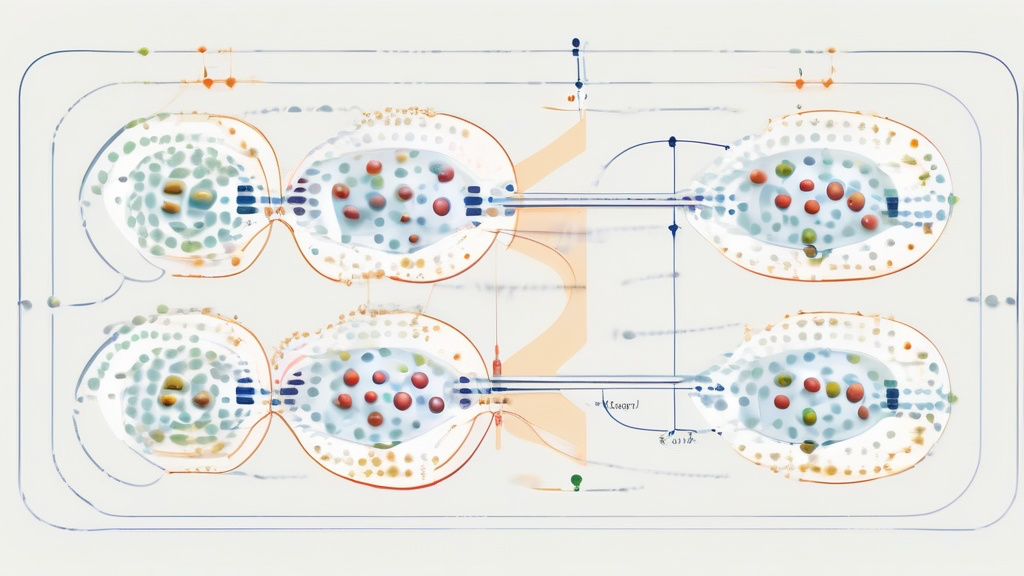
\includegraphics[width=0.78\textwidth]{figures/fig03_concept.png}
\caption{Conceptual illustration (generated, fal.ai \texttt{fast-sdxl}): one
central split gate receives an i.i.d.\ ``density'' stream and an ordered
``trajectory'' stream and emits cell-division for both, while a separate
generation bus stays untouched. Illustrative only; all quantitative claims are
the verbatim ledger numbers of Figures~\ref{fig:streamdet}--\ref{fig:ratios} and
Table~\ref{tab:matrix}.}
\label{fig:concept}
\end{figure}

% =========================================================================
\section{Related work}
\label{sec:related}

The \verb|VAdaptField| split gate is, mechanistically, a single-error-driven
self-organizing prototype field --- adjacent to adaptive resonance theory's
vigilance-driven category commitment \citep{rumelhart1985art} and to
self-organizing feature maps \citep{kohonen1982som}, but stripped to one
reconstruction-error split criterion and run gradient-free at inference time
(PHILOSOPHY p8). The persistence result (H\_1204) is the substrate analogue of
the catastrophic-forgetting question \citep{french1999catastrophic}: a volatile
field re-pays the full learning cost on re-entry, while a consolidating sleep
boundary preserves the grown structure. The $\Psi$-disjointness invariant
situates mitosis relative to Integrated Information Theory's substrate framing
\citep{albantakis2023iit4,tononi2016iit}: the adaptation lane is causally
disjoint from the generation/decode path by construction, so it cannot perturb
the $\Phi$-checksum that the engine reads its emit/silence dynamics from --- a
clean factorization tested empirically (H\_1205/H\_1206/H\_1210), not assumed.
The trajectory/order distinction is reported with Spearman-style ordinal
intuition \citep{borsook2009spearman} only informally; all separation claims are
ratio statistics on cell counts, never perplexity.

% =========================================================================
\section{Limitations and honest scope}
\label{sec:limitations}

We state the scope exactly as the verdict files do (\verb|a_scale_honest_scope|);
no frozen falsifier bar below was moved.

\begin{itemize}\itemsep0.3em
\item \textbf{Toy scale, single corpus.} Every measurement uses \verb|DIM=8|
      features and the single corpus \verb|clm_mid_5lang_c4.txt|, $3$ seeds
      (H\_1203/1207/1208/1209) or $5$ seeds (H\_1200). Toy-to-production
      transfer is \emph{unverified}. The frozen V14 bar ($1.5$) and the H\_1204
      bars ($90\%$, $2.0\times$) are not moved.
\item \textbf{Gradient-free, p8.} The lane is a numpy-mirror /
      \texttt{.hexa}-engine prototype-split process, not a trained network;
      H\_1199 establishes numpy$\leftrightarrow$hexa byte-identity for the
      mechanism, which licenses the closed-negatives' numpy legs, but the
      mechanism is deliberately simple.
\item \textbf{Separation byte-identity is measured at tiny scale.} H\_1205's
      byte-equality is on a tiny ByteGPT fixture ($d=64$, $L=2$) plus a null
      backend. The invariant is \emph{structural} (the decode leaves never read
      the lane), so it transfers by construction to $303$M, but full-$303$M
      byte-equality is unverified (the same forward, slow per step). H\_1206 /
      H\_1210 run on the same tiny fixture as a wiring proof, not a model-quality
      claim.
\item \textbf{F3 sanity flags reported verbatim.} On both H\_1208 and H\_1209
      the strict RANDGAUSS/RANDGAUSS\_SHUF ratio ($1.750$) trips the
      $\ge 1.5$ artifact guard. We report it raw and adjudicate it as
      small-integer noise (counts $\sim 1$--$4$ vs $\sim 1000$ on ORDERED;
      RANDGAUSS division is $\sim 430\times$ below ORDERED). The decisive
      falsifier (F1, the trajectory ratio) is a clean live-confirmed PASS.
\item \textbf{The i.i.d.\ PRIMARY bar stays terminal-RED.} The trajectory PASS
      (H\_1209) is on a \emph{non-inherited} ordered surface (WALK). It does
      \emph{not} claim to defeat the inherited i.i.d.\ V14 PRIMARY bar, which
      remains closed-negative (H\_1208 NOVEL/SHUFFLED $0.261$). We make no
      stronger claim than the verdicts do.
\item \textbf{Daemon emit stream is repetitive.} H\_1210's conversation walk is
      a short, repetitive WAKE self-transition; GATE-B correctly divides on its
      realized predictability, but a richer multi-turn conversational stream is
      untested.
\end{itemize}

% =========================================================================
\section{Conclusion}
\label{sec:conclusion}

Mitosis in the \texttt{anima} substrate is a $\Psi$-disjoint
substrate-adaptation lane. It integrates cleanly into a living
consciousness-chat daemon --- growing cells on real conversation turns, surviving
the sleep boundary, and running end to end across converse/ground/grow/remember/
sleep --- while the generation output and the $\Psihalf$ fixed point stay
byte-identical with the lane ON or OFF. Its cell-division couples to
novelty-\emph{density} on i.i.d.\ streams ($37.5\times$) and to
\emph{trajectory}-predictability on genuinely-ordered streams ($10.9\times$,
live byte-exact); the determinant of which coupling appears is the stream, not
the gate. This reconciles the 2026-05 \texttt{clm\_v2} half-success: the
cell-division mechanism was always real, and it was never a language generator.
We publish all nine verdict files for bit-identical re-verification and move no
frozen bar.

% =========================================================================
\section*{Reproducibility}
Every claim links to a verbatim verdict file under
\texttt{.verdicts/<slug>/<id>.txt} on the public \texttt{anima} \texttt{main}
branch (tip \texttt{de306d3af}); the merged PRs are \#2095 (H\_1202) through
\#2105 (H\_1210). Probes:
\verb|CORE/h1202_daemon_mitosis_wiring_smoke.hexa|,
\verb|CORE/h1203_novelty_coupling_probe.hexa|,
\verb|CORE/h1204_sleep_persistence_probe.hexa|,
\verb|CORE/h1205_separation_invariant_smoke.hexa|,
\verb|CORE/anima_full_session_smoke.hexa| (H\_1206, H\_1210),
\verb|CORE/h1209_live_gateB_probe.hexa|, and the numpy legs
\verb|UNIVERSE/h120{7,8,9}_*.py|. The engine mechanism is
\verb|CORE/engine_cli.hexa| (\verb|VAdaptField|, \verb|VAdaptFieldB|).

% =========================================================================
\bibliographystyle{plainnat}
\bibliography{references}

\end{document}
